\documentclass[tikz,border=12pt]{standalone}
\usepackage[T1]{fontenc}
\usepackage{mathpazo}
\usepackage{amsmath,amssymb}
\usetikzlibrary{arrows.meta, positioning, calc, decorations.pathreplacing}

\definecolor{stblue}{HTML}{7B97AD}
\definecolor{rwgold}{HTML}{B8995E}
\definecolor{sage}{HTML}{7A9A7E}
\definecolor{dkbrown}{HTML}{3D3530}
\definecolor{wmgray}{HTML}{7B7067}
\definecolor{cream}{HTML}{F9F6F0}
\definecolor{border}{HTML}{D4C9B8}
\definecolor{terracotta}{HTML}{C47A6A}

\begin{document}
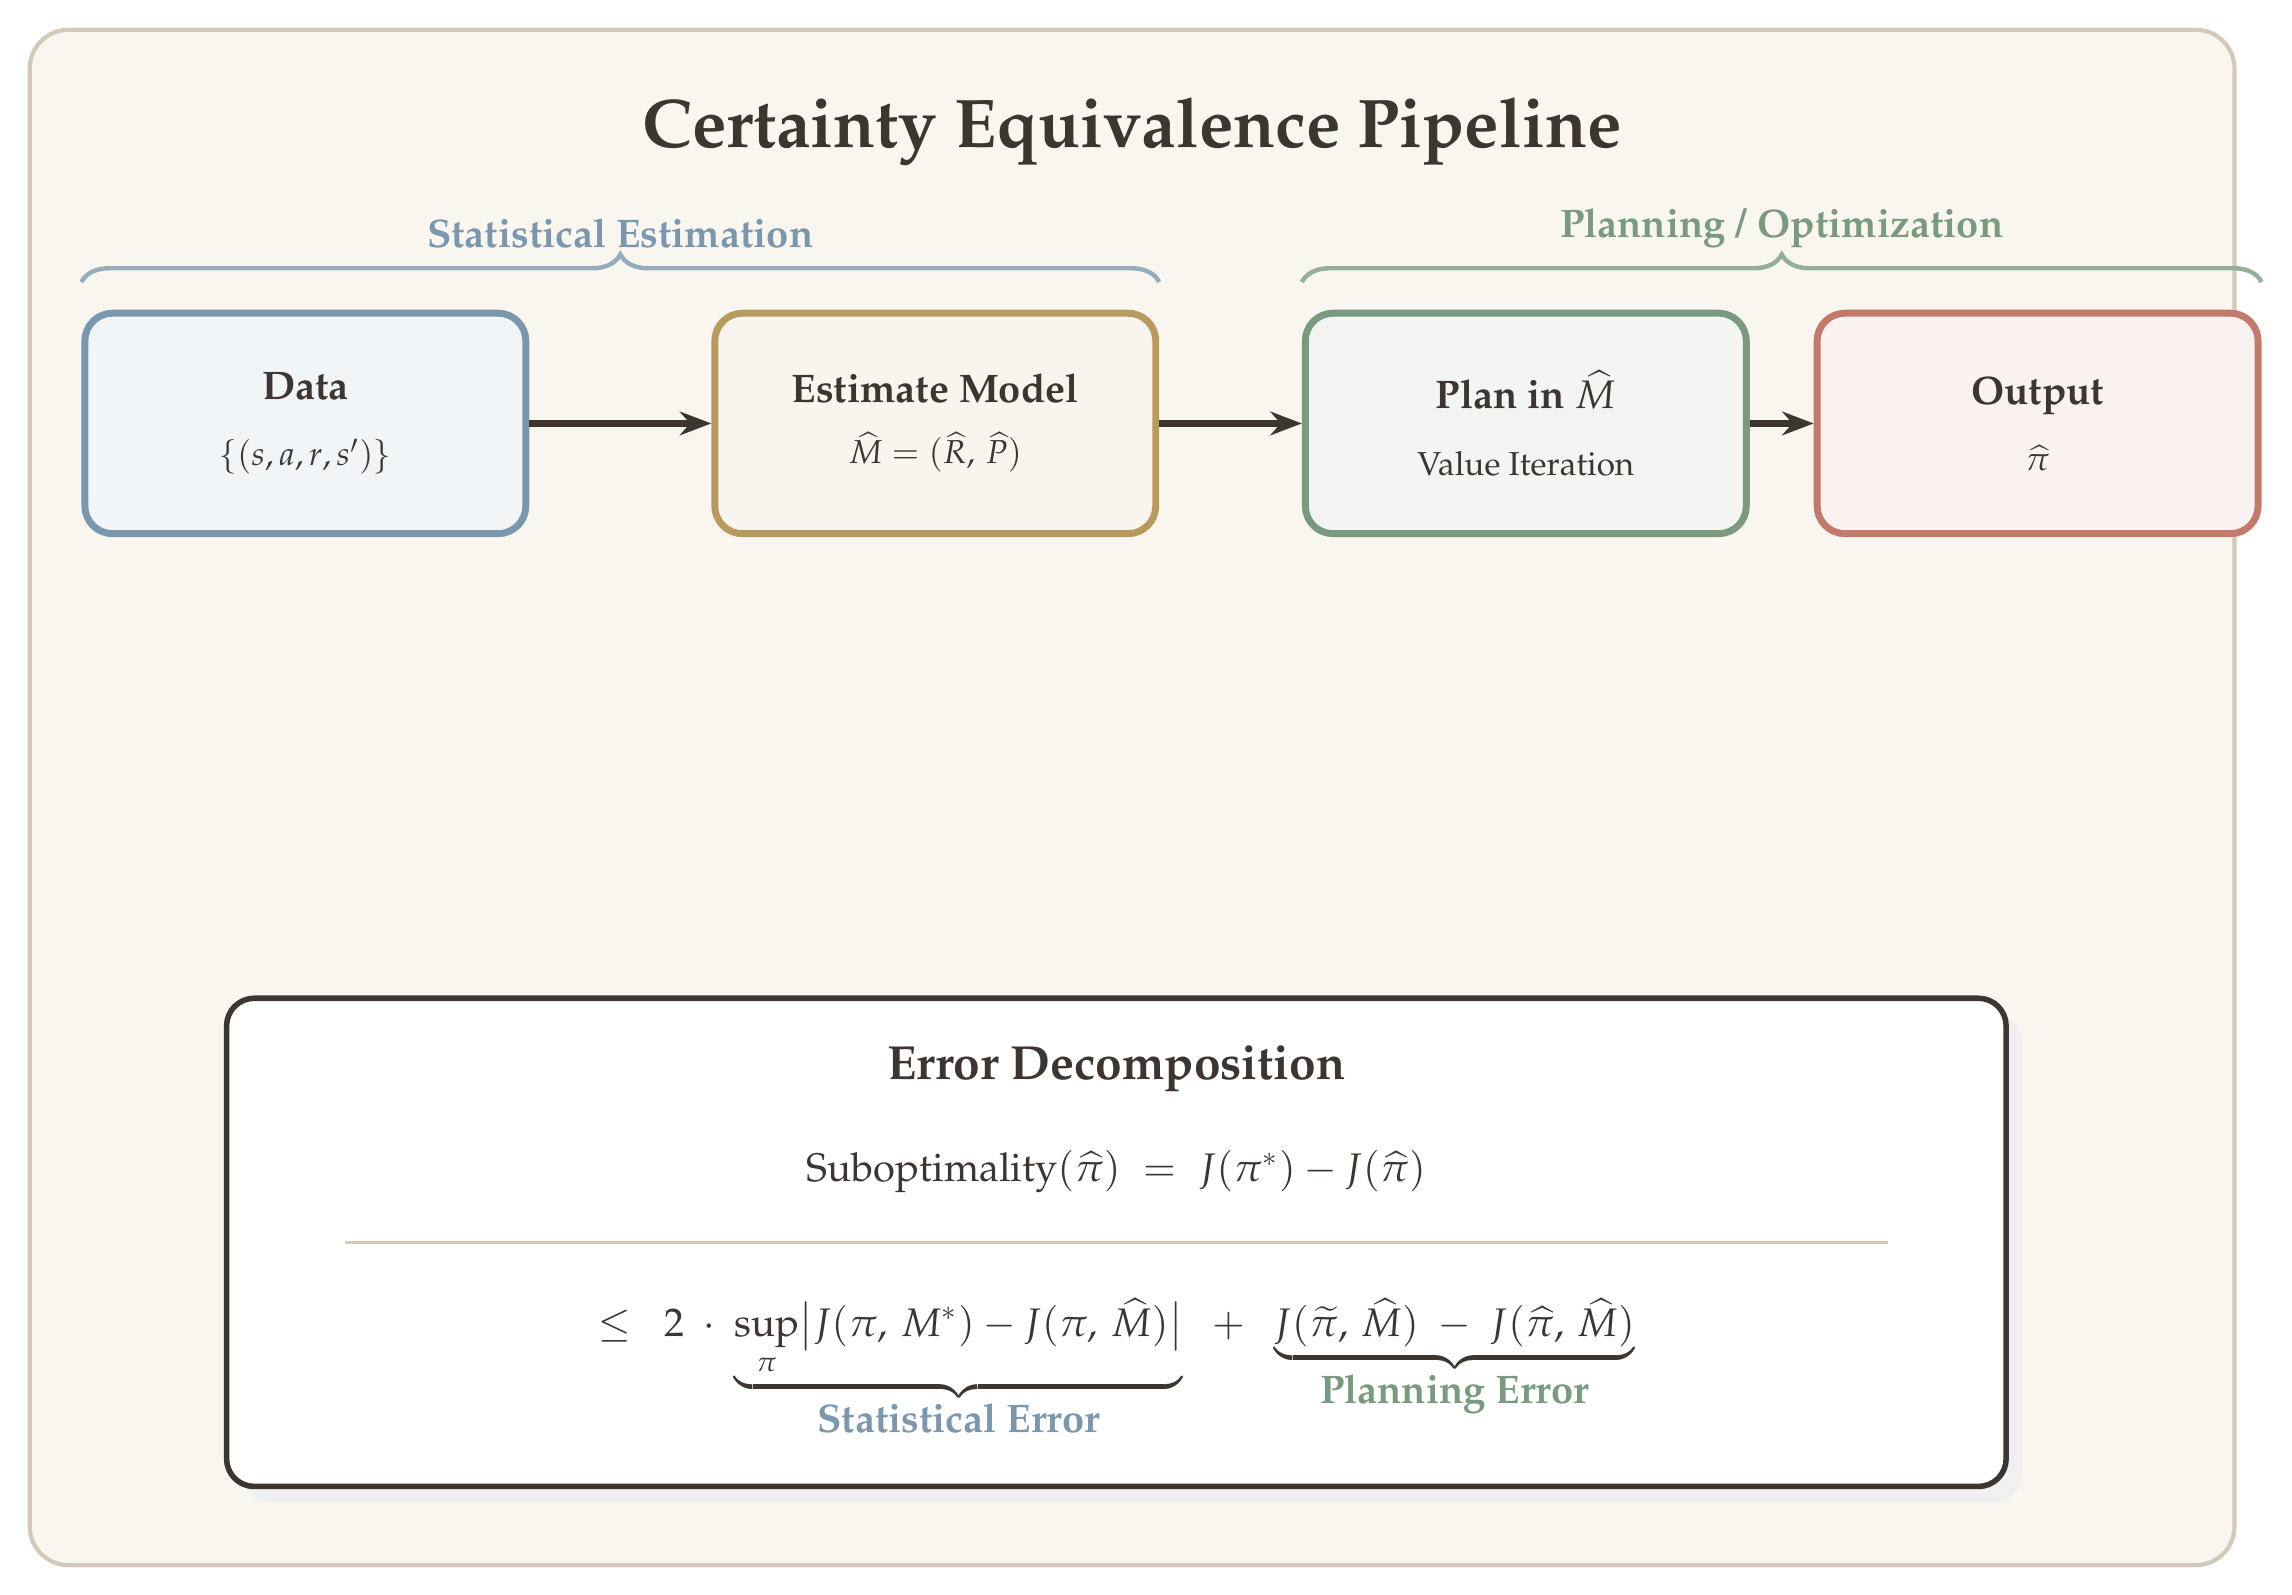
\begin{tikzpicture}[
  >={Stealth[length=4mm, width=3mm]},
  pbox/.style={
    draw=#1, line width=2.5pt, fill=#1!10, rounded corners=10pt,
    minimum width=56mm, minimum height=28mm, font=\Large, text=dkbrown,
    align=center, inner sep=8pt
  },
  arr/.style={->, line width=2.5pt, dkbrown},
  brace/.style={decorate, decoration={brace, amplitude=10pt, raise=8pt},
    line width=1.6pt, #1},
]

% Background
\fill[cream, rounded corners=14pt] (-2,-11) rectangle (26,8.5);
\draw[border, rounded corners=14pt, line width=1.5pt] (-2,-11) rectangle (26,8.5);

% Title
\node[font=\Huge\bfseries, text=dkbrown] at (12,7.2)
  {Certainty Equivalence Pipeline};

% =============================================
% Top row: 4 pipeline boxes
% =============================================

\node[pbox=stblue] (data) at (1.5,3.5)
  {\textbf{Data}\\[6pt]
   {\large $\{(s,a,r,s')\}$}};

\node[pbox=rwgold] (model) at (9.5,3.5)
  {\textbf{Estimate Model}\\[4pt]
   {\large $\widehat{M} = (\widehat{R},\, \widehat{P})$}};

\node[pbox=sage] (plan) at (17.0,3.5)
  {\textbf{Plan in $\widehat{M}$}\\[6pt]
   {\large Value Iteration}};

\node[pbox=terracotta] (output) at (23.5,3.5)
  {\textbf{Output}\\[6pt]
   {\large $\widehat{\pi}$}};

% =============================================
% Arrows between pipeline boxes
% =============================================
\draw[arr] (data.east) -- (model.west);
\draw[arr] (model.east) -- (plan.west);
\draw[arr] (plan.east) -- (output.west);

% =============================================
% Braces above boxes
% =============================================
\draw[brace=stblue!80]
  ([yshift=2pt]data.north west) -- ([yshift=2pt]model.north east)
  node[midway, above=16pt, font=\Large\bfseries, text=stblue] {Statistical Estimation};

\draw[brace=sage!80]
  ([yshift=2pt]plan.north west) -- ([yshift=2pt]output.north east)
  node[midway, above=16pt, font=\Large\bfseries, text=sage] {Planning / Optimization};

% =============================================
% Bottom section: Error decomposition
% =============================================

% Shadow
\fill[black!6, rounded corners=10pt]
  (0.7,-10.2) rectangle (23.3,-4.0);
% White box
\fill[white, rounded corners=10pt]
  (0.5,-10.0) rectangle (23.1,-3.8);
\draw[dkbrown, line width=2pt, rounded corners=10pt]
  (0.5,-10.0) rectangle (23.1,-3.8);

% Header
\node[font=\LARGE\bfseries, text=dkbrown] at (11.8,-4.7)
  {Error Decomposition};

% Suboptimality line
\node[font=\Large, text=dkbrown] at (11.8,-6.0)
  {$\mathrm{Suboptimality}(\widehat{\pi}) \;=\; J(\pi^*) - J(\widehat{\pi})$};

% Separator
\draw[border, line width=1.2pt] (2.0,-6.9) -- (21.6,-6.9);

% Bound line
\node[font=\Large, text=dkbrown] at (11.8,-8.5)
  {$\displaystyle\leq\;\; 2\;\cdot\;
   \underbrace{\sup_\pi \bigl|J(\pi,\, M^*) - J(\pi,\, \widehat{M})\bigr|}_{\textstyle\color{stblue}\textbf{Statistical Error}}
   \;\;+\;\;
   \underbrace{J(\widetilde{\pi},\, \widehat{M}) \;-\; J(\widehat{\pi},\, \widehat{M})}_{\textstyle\color{sage}\textbf{Planning Error}}$};

\end{tikzpicture}
\end{document}
